\chapter{Schwarze-Loch-Entropie, Holografie und de-Sitter-Raum}

\lectureoverview{Wir schließen das Korrespondenzargument ab, das in der vorherigen Vorlesung begonnen wurde. Die Entropie einer stark angeregten Saite ist proportional zu ihrer Masse, während die Entropie eines Schwarzschild-Schwarzen-Lochs proportional zu seiner Fläche ist. Die beiden Formeln werden nicht dadurch miteinander verknüpft, dass man ein stark gravitierendes Schwarzes Loch mit einer freien Saite gleichsetzt, sondern indem man die Stringkopplung langsam verändert, bis beide Beschreibungen zusammenpassen. Das Flächengesetz führt dann auf natürliche Weise zum holografischen Prinzip. Im letzten Teil der Vorlesung werden expandierender Raum und die de-Sitter-Geometrie eingeführt, deren Horizont in der nächsten Vorlesung untersucht wird.}

\section{Zurück zum Abzählproblem}

Bei der Abzählung langer Saiten war noch eine Frage offen. Wird eine feste Gesamtlänge auf mehrere Saiten verteilt, sind identische Saiten gleicher Länge ununterscheidbar. Ihre Positionen im Kasten gehören dennoch zum Zustand, und der Kasten wird ungefähr so groß gewählt wie der Bereich, den die entsprechende einzelne lange Saite einnimmt.

\begin{classroomqa}
\audiencequestion{Sind die kurzen Saiten voneinander unterscheidbar, und zählen ihre Positionen mit?\lecturetimestamp{00:00:37}}
\lecturerresponse{Saiten mit identischen Eigenschaften sind ununterscheidbar, ihre Positionen im Kasten werden jedoch mitgezählt. Der Vergleich erfolgt bei festem Volumen, das so gewählt ist, dass es dem von der langen Saite eingenommenen Bereich entspricht.}
\end{classroomqa}

Damit können wir nun das Ziel formulieren. Wir stellen eine kurze Liste von Gleichungen zusammen und leiten daraus die Skalierung der Schwarzen-Loch-Entropie ab. Dazu ist weder ein Integral noch eine unendliche Summe erforderlich. Die Schwierigkeit ist nicht algebraischer Art; sie besteht darin, zu erkennen, welche Größen miteinander verglichen werden dürfen und an welcher Stelle des Arguments.

\section{Natürliche Einheiten und die Planck-Fläche}

Wir setzen
\begin{equation}
c=\hbar=1,
\label{eq:l07-natural-units}
\end{equation}
, lassen aber die Newtonsche Gravitationskonstante explizit stehen. Daraus folgt zunächst, dass Zeit und Länge dieselbe Einheit haben. Die Photon-Beziehung
\begin{equation}
E=\frac{\hbar c}{\lambda}
\end{equation}
und die Masse-Energie-Beziehung \(E=mc^2\) ergeben dann
\begin{equation}
[M]=L^{-1}.
\label{eq:l07-mass-dimension}
\end{equation}
Masse lässt sich somit als inverse Länge angeben.

\begin{figure}[htbp]
\centering
\includegraphics[width=0.62\textwidth]{lecture_07_figure_02.png}
\caption{Die Konvention natürlicher Einheiten zu Beginn der Dimensionsbetrachtung. Die Energieformel wird durch die obigen Gleichungen ergänzt.}
\lectureframe{00:03:27.900}
\end{figure}

Um die Einheiten von \(G_N\) zu bestimmen, verwenden wir die Newtonsche Beschleunigung lediglich als Dimensionsbuchhaltung:
\begin{equation}
a\sim\frac{G_NM}{R^2}.
\end{equation}
Da \(T\) und \(L\) dieselben Einheiten haben, gilt \([a]=L/T^2=L^{-1}\). Zusammen mit Gleichung~\eqref{eq:l07-mass-dimension} folgt daraus
\begin{equation}
[G_N]=L^2.
\end{equation}
In diesen Einheiten hat die Newtonsche Gravitationskonstante die Dimension einer Fläche. Definiert man die Planck-Länge durch
\begin{equation}
G_N=\ell_p^2,
\label{eq:l07-planck-area}
\end{equation}
so wird unmittelbar klar, warum \(A/G_N=A/\ell_p^2\) dimensionslos ist: Der Ausdruck gibt eine Fläche in Planck-Flächen an.

\section{Die Stringkopplung und die Stärke der Gravitation}

Nun müssen wir die Gravitation in die Sprache der Stringtheorie übersetzen. Anschaulich lässt sich das als Austauschprozess auffassen. Wenn eine Saite sich selbst kreuzt, kann sie sich aufspalten und wieder verbinden. Eine kleine geschlossene Stringschleife kann von einem Objekt emittiert und von einem anderen absorbiert werden; handelt es sich bei dieser Anregung um ein Graviton, vermittelt der Prozess die Gravitation. Bei der Emission tritt ein Wechselwirkungsfaktor auf und bei der Absorption ein weiterer, sodass die Stärke des Austauschs den Faktor \(g_s^2\) enthält.

Die Kopplung \(g_s\) ist dimensionslos. Genauer gesagt ist sie eine Kopplung auf Amplitudenebene, während eine Wahrscheinlichkeit oder Rate in der Ordnung \(g_s^2\) beginnt.\editorialnote{In der Vorlesung wird \(g_s\) gelegentlich als Wahrscheinlichkeit bezeichnet und dann zu deren Quadratwurzel korrigiert. Die Störungskopplung gehört auf die Amplitudenebene.} Da \(G_N\) die Dimension einer Fläche hat, fehlt noch eine Längenskala. Diese liefert die fundamentale Stringlänge \(\ell_s\), die Skala einer elementaren Auslenkung der Saite:
\begin{equation}
G_N\sim g_s^2\ell_s^2,
\qquad
\ell_p\sim g_s\ell_s.
\label{eq:l07-planck-string}
\end{equation}

\begin{figure}[htbp]
\centering
\includegraphics[width=0.72\textwidth]{lecture_07_figure_05.png}
\caption{Die Kopplungsbeziehung an der Tafel: \(G_N=\ell_p^2\) und \(g_s^2\ell_s^2\sim\ell_p^2\).}
\lectureframe{00:12:15.000}
\end{figure}

Bei schwacher Kopplung, \(g_s\ll1\), ist die Planck-Länge viel kleiner als die Stringlänge. Wird \(g_s\) verringert, schwächt sich die Gravitation ab, während die elementare Stringskala unverändert bleibt.\editorialnote{In einer effektiven vierdimensionalen Theorie gehen auch Kompaktifizierungsdaten und numerische Konventionen in \(G_N\) ein. In diesem Skalierungsargument werden sie festgehalten und nicht weiter berücksichtigt.}

\section{Abzählung einer langen Saite}

Entropie zählt die elementaren Entscheidungen, die zur Festlegung eines Zustands erforderlich sind. Wir ersetzen eine stark angeregte Saite durch einen Weg auf einem quadratischen Gitter. An jedem Gitterpunkt kann der nächste Schritt in eine von vier Richtungen weisen. Ob man die elementare Wahl als eine Entscheidung zwischen vier Möglichkeiten oder als zwei binäre Entscheidungen beschreibt, ändert lediglich eine Konstante der Größenordnung eins. Entscheidend ist die Anzahl der Schritte.

Sei \(L\) die Konturlänge der Saite und \(\ell_s\) die Länge jedes Schritts. Dann sind
\begin{equation}
N=\frac{L}{\ell_s}
\end{equation}
Schritte erforderlich. Die Anzahl der Wege wächst exponentiell, schematisch wie \(\Omega_N\sim q^N\), wobei \(q\) von der Größenordnung eins ist. Daher gilt
\begin{equation}
S_{\mathrm{str}}=\log\Omega_N\sim N\sim\frac{L}{\ell_s}.
\label{eq:l07-string-entropy-length}
\end{equation}

\begin{figure}[htbp]
\centering
\includegraphics[width=0.68\textwidth]{lecture_07_figure_03.png}

\vspace{0.7em}
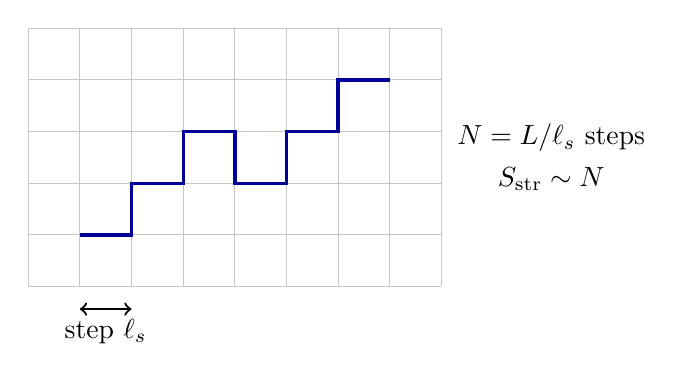
\begin{tikzpicture}[scale=0.82]
  \draw[step=0.8cm,gray!45,thin] (0,0) grid (6.4,4.0);
  \draw[very thick,blue!60!black]
    (0.8,0.8)--(1.6,0.8)--(1.6,1.6)--(2.4,1.6)--(2.4,2.4)--
    (3.2,2.4)--(3.2,1.6)--(4.0,1.6)--(4.0,2.4)--(4.8,2.4)--
    (4.8,3.2)--(5.6,3.2);
  \draw[<->,thick] (0.8,-0.35)--(1.6,-0.35);
  \node[below] at (1.2,-0.35) {step \(\ell_s\)};
  \node[align=center] at (8.1,2.0) {\(N=L/\ell_s\) steps\\[0.3em]\(S_{\mathrm{str}}\sim N\)};
\end{tikzpicture}
\caption{Das Gittermodell an der Tafel und seine bereinigte Interpretation als Zufallsweg. Die Konturlänge, nicht der Durchmesser des wirren Knäuels, bestimmt die Anzahl der Wahlmöglichkeiten.}
\lectureframe{00:17:20.000}
\end{figure}

Die Masse wird anhand derselben elementaren Segmente bestimmt. Ein Segment der Länge \(\ell_s\) hat die Massenskala
\begin{equation}
m_{\mathrm{seg}}\sim\frac{1}{\ell_s}.
\end{equation}

\begin{classroomqa}
\audiencequestion{Wird dem elementaren Segment die Länge \(\ell_s\) zugeordnet?\lecturetimestamp{00:18:56}}
\lecturerresponse{Ja. Seine charakteristische Länge ist \(\ell_s\), also ist seine charakteristische Masse in natürlichen Einheiten \(1/\ell_s\).}
\end{classroomqa}

Addiert man die Massen der \(L/\ell_s\) Segmente, erhält man
\begin{equation}
M\sim\frac{L}{\ell_s}\frac{1}{\ell_s}
=\frac{L}{\ell_s^2},
\qquad
L\sim M\ell_s^2.
\label{eq:l07-string-mass}
\end{equation}
Die kinetische und die potenzielle Energie der schwingenden Saite sind in dieser Skalierungsbeziehung zusammengefasst; eine ausführliche statistisch-mechanische Behandlung ergibt dieselbe Abhängigkeit. Einsetzen in Gleichung~\eqref{eq:l07-string-entropy-length} liefert die Stringformel, die wir benötigen:
\begin{equation}
S_{\mathrm{str}}\sim M\ell_s.
\label{eq:l07-string-entropy-mass}
\end{equation}

\begin{figure}[htbp]
\centering
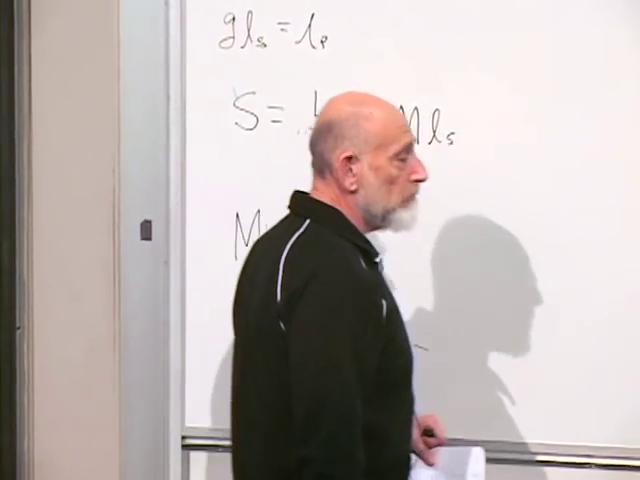
\includegraphics[width=0.66\textwidth]{lecture_07_figure_04.png}
\caption{Die Spalte für die Saite, zusammengestellt vor dem Vergleich: \(\ell_p\sim g_s\ell_s\), \(S_{\mathrm{str}}\sim L/\ell_s\sim M\ell_s\) und \(M\sim L/\ell_s^2\).}
\lectureframe{00:21:57.800}
\end{figure}

\section{Warum eine freie Saite noch kein Schwarzes Loch ist}

Auf der gravitativen Seite lautet die exakte semiklassische Formel
\begin{equation}
S_{\mathrm{BH}}=\frac{A}{4G_N}.
\label{eq:l07-bh-exact}
\end{equation}

\begin{classroomqa}
\audiencequestion{Welcher Zahlenfaktor gehört in den Nenner?\lecturetimestamp{00:23:28}}
\lecturerresponse{Vier. Das Korrespondenzargument wird die Skalierung reproduzieren, ist aber zu grob, um diesen exakten Faktor zu bestimmen.}
\end{classroomqa}

Für ein vierdimensionales Schwarzschild-Schwarzes-Loch gilt
\begin{equation}
R_s=2G_NM,
\qquad
A=4\pi R_s^2.
\end{equation}
Lässt man, wie in der Vorlesung, die numerischen Konstanten weg, erhält man
\begin{align}
S_{\mathrm{BH}}
&\sim\frac{A}{G_N}
\sim\frac{(G_NM)^2}{G_N} \\
&\sim M^2G_N
\sim M^2\ell_p^2.
\label{eq:l07-bh-scaling}
\end{align}

\begin{figure}[htbp]
\centering
\includegraphics[width=0.72\textwidth]{lecture_07_figure_06.png}
\caption{Der vollständige Vergleich an der Tafel: Die Stringentropie ist eine Länge in Stringeinheiten, während die Schwarze-Loch-Entropie eine Fläche in Planck-Einheiten ist.}
\lectureframe{00:25:35.000}
\end{figure}

Die Ähnlichkeit zwischen den Gleichungen~\eqref{eq:l07-string-entropy-mass} und \eqref{eq:l07-bh-scaling} ist suggestiv, doch es handelt sich nicht um dieselbe Formel. Es wäre falsch, das ursprüngliche Schwarze Loch einfach als freie Saite zu bezeichnen und die entsprechende Formel einzusetzen. Bei der Abzählung der freien Saite wird die anziehende Wechselwirkung zwischen ihren Teilen vernachlässigt – genau jene Wechselwirkung, die die Saite zu einem Schwarzen Loch zusammenzieht und durch negative Bindungsenergie ihre Gesamtenergie senkt.

Ein Stern macht diesen Fehler anschaulich. Ein heißes Gas mit der Masse eines Sterns in einem übergroßen Kasten ist kein Modell für einen Stern, selbst wenn die Temperatur gleich ist. Die Eigengravitation verändert die Gleichgewichtsgröße und den Zusammenhang zwischen Energie und Entropie. Jede Selbstwechselwirkung einer langen Saite einzeln zu berücksichtigen, wäre schwierig; deshalb werden wir darauf verzichten.

\begin{classroomqa}
\audiencequestion{Wenn eine kleine Schleife eine lange Saite verlässt, nimmt deren Entropie ab. Senkt der Gravitonenaustausch dann die Entropie des gravitierenden Systems?\lecturetimestamp{00:28:48}}
\lecturerresponse{Nicht beim hier betrachteten Gleichgewichtsaustausch. Virtuelle Anregungen werden in beide Richtungen emittiert und absorbiert; die Skizze zeigt keinen tatsächlichen Verlust eines dauerhaft abgespaltenen Saitenstücks. Sie soll hier lediglich die beiden Kopplungsfaktoren und damit die Abhängigkeit von \(g_s^2\) verdeutlichen.}
\end{classroomqa}

\section{Das adiabatische Korrespondenzspiel}

Beginnen wir stattdessen dort, wo die Gravitation vernachlässigbar ist. Bei \(g_s\to0\) kreuzen sich Saiten, ohne sich aufzuspalten oder zu verbinden, und die Eigengravitation verschwindet. Erhöhen wir \(g_s\) bei festgehaltenem \(\ell_s\), wird die Gravitation stärker, eine stark angeregte Saite zieht sich zusammen und wird schließlich zu einem Schwarzen Loch. Dreht man den Regler langsam zurück, muss das Schwarze Loch wieder in einen Stringzustand übergehen. Es kann sich in eine kleine Zahl langer Saiten verwandeln, doch die Hochenergie-Abzählung aus der vorherigen Vorlesung besagt, dass der dominante Sektor eine lange Saite und nicht ein riesiges Gas aus kurzen Saiten enthält.

\begin{classroomqa}
\audiencequestion{Was bleibt fest, während die Kopplung verändert wird?\lecturetimestamp{00:32:19}}
\lecturerresponse{Die Stringlänge \(\ell_s\) und damit die elementare Stringmassenskala \(1/\ell_s\) bleiben fest. Der Regler verändert \(g_s\) und damit \(G_N\sim g_s^2\ell_s^2\).}
\end{classroomqa}

Die Änderung muss langsam, isoliert und reversibel sein. Unter diesen Bedingungen ist die Entropie eine adiabatische Invariante:
\begin{equation}
\Delta S=0.
\label{eq:l07-adiabatic}
\end{equation}
Allein die Langsamkeit reicht nicht aus, wenn dissipative oder unkontrollierte Übergänge auftreten. Hier bedeutet ``adiabatisch'', dass sich dieselbe Zustandsfamilie kontinuierlich verfolgen lässt.\editorialnote{Dies ist der reversible thermodynamische Sinn von adiabatisch. Ein irreversibler Prozess kann im Sinne eines fehlenden Wärmeaustauschs adiabatisch sein und dennoch Entropie erzeugen.}

Sei die Masse des betrachteten Schwarzen Lochs \(M_0\) und seine Kopplung \(g_{s,0}\). Bevor wir das Flächengesetz verwenden, das wir erklären wollen, sagt die Dimensionsanalyse lediglich, dass die Entropie eines neutralen, nicht rotierenden Schwarzen Lochs eine Funktion der dimensionslosen Kombination
\begin{equation}
S_{\mathrm{BH}}=f(M\ell_p)
=f(Mg_s\ell_s).
\label{eq:l07-entropy-function}
\end{equation}
ist.
Bei festem \(\ell_s\) bleibt auf einem isentropen Pfad daher
\begin{equation}
Mg_s=M_0g_{s,0}
\label{eq:l07-adiabat}
\end{equation}
konstant, sofern derselbe Zustandszweig verfolgt wird.

Wenn \(g_s\) abnimmt, wird negative Bindungsenergie abgeführt, sodass die Masse \(M\) entlang dieses Pfads zunimmt. Auch die zugrunde liegende Stringkonfiguration ist weniger stark gebunden und breitet sich aus. Der formale Schwarzschildradius verhält sich auf der Adiabate jedoch wie \(R_s\sim Mg_s^2\ell_s^2\sim g_s\ell_s\) und nimmt daher ab.\editorialnote{Die mündliche Erläuterung verwendet ``wächst'' für das Objekt, das aus der gravitativen Bindung gelöst wird. Dies sollte nicht so verstanden werden, als nähme der Schwarzschildradius entlang der hergeleiteten Adiabate zu.}

\begin{classroomqa}
\audiencequestion{Wächst oder schrumpft das Objekt, wenn die Gravitation schwächer wird?\lecturetimestamp{00:36:28}}
\lecturerresponse{Seine Stringstruktur wird freigesetzt und breitet sich aus, während seine Masse zunimmt, weil die negative Bindungsenergie abgebaut wird. Der nach der Formel für Schwarze Löcher bestimmte Radius nimmt ab, bis er die Stringskala erreicht; dann ist diese Beschreibung als Schwarzes Loch nicht mehr brauchbar.}
\end{classroomqa}

\section{Zwei Kurven und ihr Schnittpunkt}

Tragen wir die Masse auf der vertikalen und die Stringkopplung auf der horizontalen Achse auf. Gleichung~\eqref{eq:l07-adiabat} beschreibt eine Hyperbel: \(M\propto g_s^{-1}\).

\begin{classroomqa}
\audiencequestion{Welche Kurve hat ein konstantes Produkt \(Mg_s\)?\lecturetimestamp{00:44:08}}
\lecturerresponse{Eine Hyperbel. Sie ist die Adiabate durch den Zielpunkt \((g_{s,0},M_0)\).}
\end{classroomqa}

Die zweite Kurve markiert den Übergang zwischen den Beschreibungen. Ein Schwarzes Loch lässt sich nicht mehr als gewöhnliche Schwarzschild-Geometrie auflösen, sobald sein Radius kleiner ist als eine elementare Auslenkung der Saite. Daher schätzen wir den Korrespondenzpunkt durch
\begin{equation}
R_s\sim\ell_s.
\label{eq:l07-correspondence-radius}
\end{equation}
Mit \(R_s\sim MG_N\) und Gleichung~\eqref{eq:l07-planck-string} wird daraus
\begin{equation}
Mg_s^2\ell_s^2\sim\ell_s,
\qquad
Mg_s^2\sim\frac{1}{\ell_s}.
\label{eq:l07-transition-curve}
\end{equation}
Die Übergangskurve fällt also wie \(M\propto g_s^{-2}\) und damit steiler als die Adiabate.

\begin{figure}[htbp]
\centering
\includegraphics[width=0.70\textwidth]{lecture_07_figure_07.png}

\vspace{0.6em}
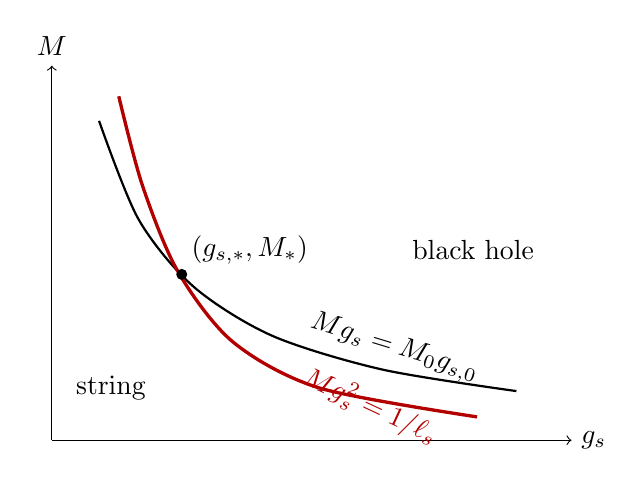
\begin{tikzpicture}[x=1cm,y=0.78cm]
  \draw[->] (0.4,0.4)--(7.0,0.4) node[right] {\(g_s\)};
  \draw[->] (0.4,0.4)--(0.4,6.5) node[above] {\(M\)};
  \draw[thick,black] plot[smooth] coordinates {(1.0,5.6) (1.5,4.0) (2.2,2.9) (3.2,2.1) (4.6,1.55) (6.3,1.2)};
  \draw[very thick,red!70!black] plot[smooth] coordinates {(1.25,6.0) (1.55,4.55) (2.0,3.15) (2.7,2.0) (3.8,1.25) (5.8,0.78)};
  \fill (2.05,3.1) circle (2pt) node[above right] {\((g_{s,*},M_*)\)};
  \node[black,rotate=-17] at (4.75,1.9) {\(Mg_s=M_0g_{s,0}\)};
  \node[red!70!black,rotate=-25] at (4.45,0.95) {\(Mg_s^2=1/\ell_s\)};
  \node at (5.75,3.5) {black hole};
  \node at (1.15,1.25) {string};
\end{tikzpicture}
\caption{Das Diagramm an der Tafel und seine bereinigte Interpretation. Die schwarze Adiabate schneidet die steiler verlaufende rote Korrespondenzkurve an dem Punkt, an dem das Objekt stringartig wird.}
\lectureframe{00:49:35.000}
\end{figure}

Am Schnittpunkt \((M_*,g_{s,*})\) lauten die beiden Gleichungen
\begin{align}
M_*g_{s,*} &= M_0g_{s,0}, \\
M_*g_{s,*}^2 &\sim \frac{1}{\ell_s}.
\end{align}
Wir quadrieren die erste Gleichung und dividieren durch die zweite:
\begin{equation}
M_*
\sim M_0^2g_{s,0}^2\ell_s.
\end{equation}
Multiplizieren wir mit \(\ell_s\), so erhalten wir
\begin{equation}
M_*\ell_s
\sim M_0^2g_{s,0}^2\ell_s^2
\sim M_0^2G_{N,0}.
\label{eq:l07-crossover-result}
\end{equation}

\begin{figure}[htbp]
\centering
\includegraphics[width=0.68\textwidth]{lecture_07_figure_08.png}
\caption{Die abgeschlossene Rechnung für den Übergang, einschließlich \(M_*\ell_s=M_0^2g_{s,0}^2\ell_s^2=M_0^2G_{N,0}\).}
\lectureframe{00:54:40.000}
\end{figure}

\begin{classroomqa}
\audiencequestion{Wenn man die beiden Kurvengleichungen dividiert, steht \(\ell_s\) dann im Zähler oder im Nenner?\lecturetimestamp{00:52:41}}
\lecturerresponse{Im Zähler. Die Division durch \(1/\ell_s\) ist eine Multiplikation mit \(\ell_s\). Daher gilt \(M_*\sim M_0^2g_{s,0}^2\ell_s\).}
\end{classroomqa}

Am Übergangspunkt gilt die Stringformel, also
\begin{equation}
S_*\sim M_*\ell_s.
\end{equation}
Die Entropie hat sich entlang des Pfads nicht verändert. Zusammen mit Gleichung~\eqref{eq:l07-crossover-result} ergibt sich daraus die Entropie des ursprünglichen Ziel-Schwarzen-Lochs:
\begin{equation}
S_{\mathrm{BH}}(M_0)
\sim M_0^2G_{N,0}
\sim M_0^2\ell_{p,0}^2.
\label{eq:l07-final-correspondence}
\end{equation}
Dies ist die gesuchte Flächengesetz-Skalierung.

\section{Was die Korrespondenz beweist und was nicht}

Diese Konstruktion besagt nicht, dass das ursprüngliche, stark gravitierende Schwarze Loch eine freie Saite ist. Sie führt das Objekt in einen Bereich, in dem die String-Abzählung verlässlich ist, bestimmt dort die Entropie und überträgt sie entlang eines reversiblen Pfads zurück. Der Übergang ist ein Crossover und keine scharf lokalisierte Phasengrenze. Deshalb kann diese Abschätzung den Koeffizienten \(1/4\) in Gleichung~\eqref{eq:l07-bh-exact} nicht bestimmen.

Dieselbe Logik funktioniert in ihrer parametrischen Form dennoch auch für geladene Schwarze Löcher, Schwarze Objekte in anderen Dimensionen und ausgedehnte Schwarze Branen. In Beispielen mit mehr Symmetrie und Supersymmetrie sind geschützte Zustandsabzählungen möglich, die bei veränderlicher Kopplung exakte Informationen bewahren. Solche Methoden liefern auch die numerischen Koeffizienten, erfordern aber mathematische Hilfsmittel, die für das vorliegende konzeptionelle Argument nicht nötig sind.

Vor allem liefert die Rechnung eine mikroskopische Deutung. Entropie ist ein Hinweis auf verborgene Struktur. Die Strömungsmechanik beschreibt Dichte, Druck und Strömung, ohne Moleküle zu berücksichtigen; die Entropie des Fluids zeigt, dass solche mikroskopischen Freiheitsgrade existieren. Allgemeine Relativitätstheorie beschreibt den Horizont ebenfalls, ohne seine Mikrozustände darzustellen. Die String-Abzählung zeigt, dass eine konsistente Quantentheorie der Gravitation genügend Zustände enthalten kann, um die Schwarze-Loch-Entropie zu erklären.

\begin{classroomqa}
\audiencequestion{Was hätte \(S\sim M^3\ell_p^3\) statt des quadratischen Ergebnisses bedeutet?\lecturetimestamp{00:59:41}}
\lecturerresponse{Das hätte wie ein Volumengesetz ausgesehen. Die Entropie gewöhnlicher Materie in einem Raum oder in einer Tasse Kaffee ist proportional zum Volumen. Das quadratische Ergebnis ist besonders, weil es über \(R_s\sim M\ell_p^2\) proportional zur Horizontfläche ist.}
\end{classroomqa}

Das Ergebnis ist ein Hinweis darauf, dass die Bekenstein--Hawking-Entropie nicht bloß eine formale thermodynamische Analogie ist. Sie deutet auf mikroskopische gravitative Freiheitsgrade hin, auch wenn die elementare Herleitung diese Freiheitsgrade nicht einzeln sichtbar macht.

\section{Von der maximalen Entropie zur Holografie}

Nun stellen wir eine andere Frage. Statt nach der Entropie eines bestimmten Zustands zu fragen, fragen wir nach der größtmöglichen Entropie, die mit einem Gebiet vereinbar ist.

Wir beginnen mit einem gewöhnlichen Gittermodell eines Raums. Wir unterteilen das Volumen in Zellen mit dem Volumen \(V_{\mathrm{cell}}\) und ordnen jeder Zelle eine Ja-Nein-Frage zu: besetzt oder leer. Susskind gibt dem imaginären Atom den bewusst absurden Namen ``''meatonium, damit keine realistischen atomaren Details von der Abzählung ablenken. Wenn
\begin{equation}
N=\frac{V}{V_{\mathrm{cell}}},
\end{equation}
gilt, sind die Anzahl der Konfigurationen und die maximale Entropie
\begin{equation}
\Omega=2^N,
\qquad
S_{\max}=\log\Omega=N\log2
\sim\frac{V}{V_{\mathrm{cell}}}.
\label{eq:l07-volume-count}
\end{equation}

\begin{figure}[htbp]
\centering
\includegraphics[width=0.68\textwidth]{lecture_07_figure_09.png}
\caption{Der Raum ist in Zellen mit je zwei Zuständen unterteilt. Damit wird eine maximale Entropie gezählt, nicht die Entropie des ordentlichen Raums, in dem die Vorlesung stattfindet.}
\lectureframe{01:05:20.000}
\end{figure}

Der tatsächliche Raum liegt weit unterhalb dieses Maximums. Ein Zustand, der all diese Zellmöglichkeiten chaotisch ausschöpfte, wäre extrem heiß. Aus dem Spielzeugmodell bleibt die gewöhnliche Erwartung, dass die Anzahl unabhängiger Freiheitsgrade und damit die maximale Entropie mit dem Volumen skaliert.

Die Gravitation stellt diese Erwartung auf den Kopf. Betrachten wir ein kugelförmiges Gebiet mit der Randfläche \(A\), der Anfangsentropie \(S_{\mathrm{i}}\) und der Masse \(M\), die kleiner ist als die Masse \(M_{\mathrm{BH}}\) eines Schwarzen Lochs, das die Kugel gerade ausfüllen würde. Wäre \(M\) größer, reichte sein Horizont bereits über den gewählten Rand hinaus.

Nun schicken wir eine Hülle mit der Masse \(M_{\mathrm{BH}}-M\) hinein. Ihre Zusammensetzung ist unerheblich; laut Vorlesung kann sie aus Licht, gewöhnlicher Materie oder sogar Schweizer Käse bestehen. Wir lassen sie kollabieren. Im Endzustand entsteht ein Schwarzes Loch, dessen Horizont das Gebiet gerade ausfüllt und dessen Entropie
\begin{equation}
S_{\mathrm{f}}=\frac{A}{4G_N}.
\end{equation}
beträgt. Der zweite Hauptsatz verlangt
\begin{equation}
S_{\mathrm{i}}\le S_{\mathrm{f}}
=\frac{A}{4G_N}.
\label{eq:l07-holographic-bound}
\end{equation}

\begin{figure}[htbp]
\centering
\includegraphics[width=0.70\textwidth]{lecture_07_figure_10.png}

\vspace{0.5em}
\begin{tikzpicture}[scale=0.88]
  \draw[thick] (0,0) circle (1.35);
  \draw[very thick,red!70!black] (0,0) circle (2.05);
  \fill[gray!25] (0,0) circle (1.32);
  \node at (0,0) {\(M,S_{\mathrm{i}}\)};
  \draw[-{Latex[length=3mm]},thick,red!70!black] (3.5,0)--(2.15,0);
  \node[align=center,right] at (3.5,0) {incoming shell\\\(M_{\mathrm{BH}}-M\)};
  \node[below] at (0,-2.2) {final horizon area \(A\)};
\end{tikzpicture}
\caption{Die Konstruktion mit der Hülle. Es wird genügend zusätzliche Masse nach innen geschickt, um ein Schwarzes Loch zu bilden, dessen Horizont das gewählte Gebiet gerade ausfüllt.}
\lectureframe{01:13:30.000}
\end{figure}

Da ein Schwarzes Loch dieser Größe ein zulässiger Zustand ist und die Ungleichung sättigt, ist die maximale Entropie
\begin{equation}
S_{\max}=\frac{A}{4G_N}.
\label{eq:l07-holographic-maximum}
\end{equation}
Dies ist das holografische Prinzip in seiner Zählform: Die maximale Anzahl unabhängiger Freiheitsgrade in einem gravitierenden Gebiet skaliert mit der Fläche seines Randes, ungefähr mit einem Freiheitsgrad der Größenordnung eins pro Planck-Fläche, und nicht mit der Anzahl der Planck-Volumina im Inneren.\editorialnote{Das Argument mit der Hülle setzt voraus, dass sich das Gebiet auf die beschriebene Weise einschließen und kollabieren lässt. Für allgemeinere Raumzeiten sind kovariante Entropiegrenzen erforderlich; das Kugelargument erfasst jedoch das in der Vorlesung verwendete Prinzip.}

Der Unterschied ist enorm. Die Intuition der lokalen Feldtheorie legt nahe, dass sich Wahlmöglichkeiten an verschiedenen inneren Punkten unabhängig kombinieren lassen, was zu einem Volumengesetz führen würde. Die Gravitation besagt, dass eine hinreichend große Zahl solcher Wahlmöglichkeiten selbst kollabieren würde; das Schwarze Loch liefert die größere zulässige Entropie. Die Zählung am Rand ist daher keine kleine Korrektur der Volumenzählung, sondern eine andere Organisation des Hilbert-Raums.

\begin{classroomqa}
\audiencequestion{Was geschieht in einem sehr großen Universum mit annähernd gleichmäßiger Dichte?\lecturetimestamp{01:15:48}}
\lecturerresponse{Diese Frage erfordert Kosmologie statt der statischen Kugelkonstruktion. Sie führt unmittelbar zu den expandierenden Lösungen der Einsteinschen Gleichungen.}
\end{classroomqa}

\begin{classroomqa}
\audiencequestion{Gibt es einen Zusammenhang zwischen der Flächengrenze und der Unschärferelation?\lecturetimestamp{01:16:03}}
\lecturerresponse{Die Vorlesung lässt diese Frage offen und wendet sich als Nächstes der Kosmologie zu.}
\end{classroomqa}

\section{Expandierender Raum}

Wir leiten die kosmologischen Lösungen der Einsteinschen Gleichungen hier nicht her, sondern schreiben sie hin und lernen, sie zu lesen. Räumliche Schnitte können positiv gekrümmt und geschlossen, negativ gekrümmt und hyperbolisch oder flach sein. Für die vorliegende Diskussion betrachten wir in einer zeitabhängigen Raumzeit räumliche, flache euklidische Schnitte.

\begin{classroomqa}
\audiencequestion{Was ist das Analogon des gewöhnlichen euklidischen Raums für die Raumzeit?\lecturetimestamp{01:19:37}}
\lecturerresponse{Der Minkowski-Raum. Die hier betrachtete Kosmologie hat flache räumliche Schnitte, ist aber keine Minkowski-Raumzeit, denn ihre räumliche Metrik ändert sich mit der Zeit.}
\end{classroomqa}

Das bekannte Bild eines Ballons beschreibt eine expandierende, geschlossene Fläche in einer Dimension weniger. Susskind erinnert sich an einen Versuch mit einem großen, markierten Ballon: Der Marker schwächte das Gummi, und der Ballon platzte mit einem Knall. Das Missgeschick macht auch einen begrifflichen Mangel der Analogie deutlich. Wenn ein gewöhnlicher Ballon expandiert, entfernen sich seine Gummimoleküle voneinander und das Material wird dünner, bis es reißt. Die lokalen Naturgesetze werden im kosmologischen Raum nicht verdünnt. Damit die Analogie erhalten bleibt, müsste man sich vorstellen, dass ständig neue Gummimoleküle eingefügt werden, sodass jede kleine Region dieselben lokalen Eigenschaften behält. In einem flachen Modell ersetzen wir den Ballon durch eine große Fläche, die gleichmäßig nach außen gezogen und auf ähnliche Weise fortlaufend ergänzt wird.

Mathematisch geht die Expansion in die Metrik ein:
\begin{equation}
\begin{aligned}
ds^2&=-dt^2+a(t)^2d\mathbf{x}^2,\\
d\mathbf{x}^2&=\delta_{ij}\,dx^i dx^j
=dx^2+dy^2+dz^2.
\end{aligned}
\label{eq:l07-frw-metric}
\end{equation}

\begin{figure}[htbp]
\centering
\includegraphics[width=0.72\textwidth]{lecture_07_figure_11.png}
\caption{Die räumlich flache Expansionsmetrik in der Form, in der sie an der Tafel angeschrieben wurde.}
\lectureframe{01:25:10.000}
\end{figure}

Punkte mit festen räumlichen Koordinaten heißen komovierend. Haben zwei solche Punkte den Koordinatenabstand \(\Delta x\), so beträgt ihr Eigenabstand zum Zeitpunkt \(t\)
\begin{equation}
D(t)=a(t)\Delta x.
\label{eq:l07-proper-distance}
\end{equation}
Ihre Koordinaten bewegen sich nicht, aber der metrische Abstand zwischen ihnen ändert sich. Leiten wir bei festem \(\Delta x\) ab, so erhalten wir
\begin{equation}
V=\dot D=\dot a\,\Delta x
=\frac{\dot a}{a}D.
\end{equation}
Wir definieren den Hubble-Parameter durch
\begin{equation}
H(t)=\frac{\dot a(t)}{a(t)}.
\label{eq:l07-hubble-parameter}
\end{equation}
Dann gilt
\begin{equation}
V=H(t)D,
\label{eq:l07-hubble-law}
\end{equation}
Dies ist das Hubble-Gesetz zu einem festen kosmischen Zeitpunkt.

\begin{figure}[htbp]
\centering
\includegraphics[width=0.68\textwidth]{lecture_07_figure_12.png}
\caption{Das Abstands-Rezessions-Gesetz für gleiche Zeiten an der Tafel: \(V=D\,\dot a/a\).}
\lectureframe{01:29:10.000}
\end{figure}

Die Bezeichnung ``''Hubble-Konstante kann irreführend sein. Im Allgemeinen ändert sich \(H(t)\) mit der Zeit. Räumlich konstant ist das Verhältnis \(V/D\) für jedes Paar komovierender Punkte auf derselben Zeitscheibe.

\begin{classroomqa}
\audiencequestion{Bei weit entfernten Galaxien: Auf welchen Zeitpunkt bezieht sich diese Relation? Wir beobachten sie zu einer früheren Epoche.\lecturetimestamp{01:31:10}}
\lecturerresponse{Gleichung~\eqref{eq:l07-hubble-law} ist eine Aussage für gleiche Zeiten. Eine Beobachtung folgt einem lichtartigen, in die Vergangenheit gerichteten Strahl und erfasst die entfernte Galaxie zu einem früheren Zeitpunkt. Der Zusammenhang zwischen gemessener Rotverschiebung und Entfernung erfordert daher die vollständige Geschichte entlang des Lichtkegels und nicht nur einen momentanen Wert von \(H\).}
\end{classroomqa}

\begin{figure}[htbp]
\centering
\includegraphics[width=0.66\textwidth]{lecture_07_figure_13.png}
\caption{Die Raumzeit-Skizze veranschaulicht den Unterschied zwischen einem Abstand zu gleicher Zeit und dem, was ein Beobachter entlang eines in die Vergangenheit gerichteten Lichtstrahls sieht.}
\lectureframe{01:33:20.000}
\end{figure}

\section{Die Hubble-Skala und die de-Sitter-Expansion}

In Einheiten mit \(c=1\) ergibt Gleichung~\eqref{eq:l07-hubble-law} für den Abstand
\begin{equation}
D_H=\frac{1}{H}.
\label{eq:l07-hubble-radius}
\end{equation}
eine Rezessionsgeschwindigkeit von eins. Komovierende Punkte in größerer Entfernung können \(V>1\) oder sogar \(V\gg1\) haben, ohne die spezielle Relativitätstheorie zu verletzen. Sie bewegen sich nicht schneller als Licht an einem lokalen Beobachter vorbei; ihr Eigenabstand wächst, weil die Geometrie dazwischen expandiert.\editorialnote{In einer allgemeinen zeitabhängigen Kosmologie ist \(1/H\) der Hubble-Radius und nicht automatisch ein Ereignishorizont. Im anschließend behandelten de-Sitter-Fall ist er die konstante Horizontskala.}

In vielen älteren, abgebremsten kosmologischen Modellen nimmt \(H(t)\) ab und \(1/H(t)\) zu, sodass Regionen, die sich einst überlichtschnell voneinander entfernten, später kausal in Kontakt treten können. Das in der Vorlesung besprochene Bild für späte Zeiten nähert sich stattdessen einem positiven konstanten Wert \(H\). Dann bleibt \(1/H\) fest, und die Expansionsgleichung lautet
\begin{equation}
\frac{\dot a}{a}=H,
\qquad
\dot a=Ha.
\label{eq:l07-constant-h}
\end{equation}

\begin{classroomqa}
\audiencequestion{Welche Einheit hat ein konstanter Hubble-Parameter?\lecturetimestamp{01:38:24}}
\lecturerresponse{Der Kehrwert einer Zeit. Bei \(c=1\) entspricht das dem Kehrwert einer Länge. Die Größe \(H^{-1}\) gibt sowohl eine Expansionszeit als auch eine Entfernungsskala an; in der Vorlesung dient etwa fünfzehn Milliarden Jahre als Größenordnungsbeispiel.}
\end{classroomqa}

Die Lösung von Gleichung~\eqref{eq:l07-constant-h} lautet
\begin{equation}
a(t)=a_0e^{Ht}.
\label{eq:l07-desitter-scale-factor}
\end{equation}

\begin{classroomqa}
\audiencequestion{Welche Funktion hat eine Änderungsrate, die proportional zu ihr selbst ist?\lecturetimestamp{01:39:04}}
\lecturerresponse{Eine Exponentialfunktion. Der Skalenfaktor ist also \(a_0e^{Ht}\), während der räumliche Koeffizient \(a(t)^2\) in der Metrik wie \(e^{2Ht}\) wächst.}
\end{classroomqa}

\begin{figure}[htbp]
\centering
\includegraphics[width=0.70\textwidth]{lecture_07_figure_14.png}
\caption{Die Gleichungen mit konstantem \(H\) und ihre exponentielle Lösung an der Tafel.}
\lectureframe{01:39:30.000}
\end{figure}

Eine Raumzeit mit dieser exponentiellen Expansion ist der de-Sitter-Raum. Seine konstante Hubble-Skala erzeugt einen Ereignishorizont in endlichem Eigenabstand. In gewissem Sinne bildet die Geometrie das Gegenstück zum Bild des Schwarzen Lochs: Ein Beobachter bleibt innerhalb eines kosmologischen Horizonts, während sich hinreichend weit entfernte Objekte entfernen und keine Signale senden können, die den Beobachter noch erreichen. Ein Horizont des Schwarzen Lochs verbirgt dessen Inneres vor einem äußeren Beobachter; ein de-Sitter-Horizont verbirgt das Äußere des für den Beobachter zugänglichen Bereichs. Anders als ein gewöhnliches verdampfendes Schwarzes Loch wird die ideale de-Sitter-Geometrie hier als fortbestehend betrachtet. Der Vergleich beginnt hier erst. Die nächste Vorlesung behandelt den Horizont, seine Thermodynamik und die Rätsel, die er für die Kosmologie aufwirft.
